\documentclass{article}
\usepackage[utf8]{inputenc}
% \usepackage{ctex}
\usepackage[letterpaper,top=2cm,bottom=2cm,left=3cm,right=3cm,marginparwidth=1.75cm]{geometry}

% Useful packages
\usepackage{amsmath}
\usepackage{graphicx}
\usepackage[colorlinks=true, allcolors=blue]{hyperref}

%%%%%%%%%%%%%%%%%%%%%%%%%%%%%
%%%%%%%%%%%%%%%%%%%%%%%%%%%%%
%%%% Import the package %%%%%
%%%%%%%%%%%%%%%%%%%%%%%%%%%%%
%%%%%%%%%%%%%%%%%%%%%%%%%%%%%
\usepackage{tikz}
\usepackage{tikz-3dplot}

\title{tikz}
\author{keke}

\begin{document}
\maketitle

\section{History}
The original German text of TikZ is TikZ ist kein Zeichenprogramm, which is a recursive acronym for "GNU's Not Unix!".

There are many tikz examples on this site: https://texample.net/tikz/examples/

Some other starters:
\begin{itemize}
    \item https://www.overleaf.com/learn
    \item https://github.com/Hansimov/pgfmanual-zh
\end{itemize}

\section{Basic Commands}
%%%%%%%%%%%%%%%%%%%%%%%%%%%%%
%%%%%%%%%%%%%%%%%%%%%%%%%%%%%
%%%% Let's start drawing %%%%
%%%%%%%%%%%%%%%%%%%%%%%%%%%%%
%%%%%%%%%%%%%%%%%%%%%%%%%%%%%
% use \begin to tell latex you are using tikz.
% use \draw to start your stroke, and use semicolon to end it.
% first bracket: (starting x, starting y)
% use special commands to simplify your drawing
% use extra arguments to beautify your drawing
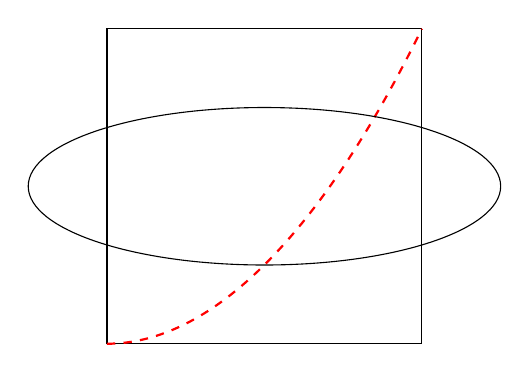
\begin{tikzpicture}
\draw (0,0) -- (4,0) -- (4,4) -- (0,4) -- cycle;
\draw (0,0) [red,thick,dashed] parabola (4,4);
\draw (2,2) ellipse (3cm and 1cm);
\end{tikzpicture}\newline
% use grid when necessary, or confused
% use fill to give it color, ! means a color mixture (You will see it much more often in VG100 manual's section)
% REMEMBER: make a clear illustration. I personally do not encourage fancy colors in latex.
% use \arc properly.
% e.g.: arc (starting angle, ending angle, radius)
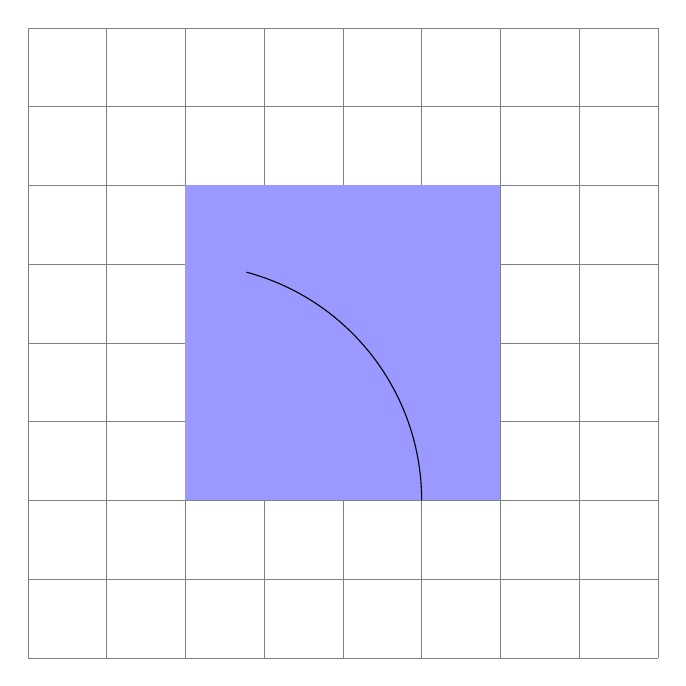
\begin{tikzpicture}
\draw[step=1cm,gray,very thin] (-2,-2) grid (6,6);
\fill[blue!40] (0,0) rectangle (4,4);
\draw (3,0) arc (0:75:3cm);
\end{tikzpicture}\newline
% add node (explanatory texts) in certain places
% The node command creates a label at the specified coordinate, which in this case is above the top center of the rectangle.
% Greatly improve the readability
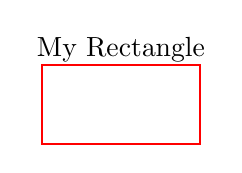
\begin{tikzpicture}
\draw[red, thick] (0,0) rectangle (2,1);
\node at (1,1.2) {My Rectangle};
\end{tikzpicture}

\section{Advanced tikz}
%%%%%%%%%%%%%%%%%%%%%%%%%%%%%
%%%%%%%%%%%%%%%%%%%%%%%%%%%%%
%%%%% Advanced drawing %%%%%%
%%%%%%%%%%%%%%%%%%%%%%%%%%%%%
%%%%%%%%%%%%%%%%%%%%%%%%%%%%%
% let's explore some more advanced TikZ features.
% Here's an example of a flowchart:
% Remember to use "\usetikzlibrary{...}"
\usetikzlibrary{positioning, shapes.geometric}
\begin{tikzpicture}[node distance=10pt]
  \node[draw, rounded corners]                        (start)   {Start};
  \node[draw, below=of start]                         (step 1)  {Step 1};
  \node[draw, below=of step 1]                        (step 2)  {Step 2};
  \node[draw, diamond, aspect=2, below=of step 2]     (choice)  {Choice};
  \node[draw, right=30pt of choice]                   (step x)  {Step X};
  \node[draw, rounded corners, below=20pt of choice]  (end)     {End};

  \draw[->] (start)  -- (step 1);
  \draw[->] (step 1) -- (step 2);
  \draw[->] (step 2) -- (choice);
  \draw[->] (choice) -- node[left]  {Yes} (end);
  \draw[->] (choice) -- node[above] {No}  (step x);
  \draw[->] (step x) -- (step x|-step 2) -> (step 2);
\end{tikzpicture} \newline
% more fancy stuffs
% learn by yourself on
\usetikzlibrary{shapes.geometric}
\usetikzlibrary{arrows.meta,arrows}
\begin{tikzpicture}
[auto,
decision/.style={diamond, draw=blue, thick, fill=blue!20,
text width=4.5em,align=flush center,
inner sep=1pt},
block/.style ={rectangle, draw=blue, thick, fill=blue!20,
text width=5em,align=center, rounded corners,
minimum height=4em},
line/.style ={draw, thick, -latex',shorten >=2pt},
cloud/.style ={draw=red, thick, ellipse,fill=red!20,
minimum height=2em}]
\matrix [column sep=5mm,row sep=7mm]
{
% row 1
\node [cloud] (expert) {expert}; &
\node [block] (init) {initialize model}; &
\node [cloud] (system) {system}; \\
% row 2
& \node [block] (identify) {identify candidate model}; & \\
% row 3
\node [block] (update) {update model}; &
\node [block] (evaluate) {evaluate candidate models}; & \\
% row 4
& \node [decision] (decide) {is best candidate}; & \\
% row 5
& \node [block] (stop) {stop}; & \\
};
\begin{scope}[every path/.style=line]
\path (init) -- (identify);
\path (identify) -- (evaluate);
\path (evaluate) -- (decide);
\path (update) |- (identify);
\path (decide) -| node [near start] {yes} (update);
\path (decide) -- node [midway] {no} (stop);
\path [dashed] (expert) -- (init);
\path [dashed] (system) -- (init);
\path [dashed] (system) |- (evaluate);
\end{scope}
\end{tikzpicture}\newpage

We can also create more complex shapes using the path command, which allows us to specify a sequence of points through which the path should pass. Here's an example of a spiral:

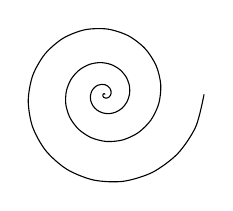
\begin{tikzpicture}
    \draw [domain=0:25.1327,variable=\t,smooth,samples=75]
        plot ({\t r}: {0.002*\t*\t});
\end{tikzpicture}

This code creates a spiral by plotting a parametric function, where r converts degrees to radians and 0.05 determines the distance between each turn of the spiral.
Another example is to use tikz to draw 3D pic.

The code then draws the x, y, and z axes using the thick and -> options to make them stand out and indicate their direction. The cube itself is drawn using the draw and fill options to create the edges and faces, respectively.Finally, dashed lines are added to indicate the hidden edges of the cube that are not visible from the current viewpoint.

\tdplotsetmaincoords{60}{110}
\begin{tikzpicture}[scale=2, tdplot_main_coords]
  \draw[thick,->] (0,0,0) -- (1,0,0) node[anchor=north east]{$x$};
  \draw[thick,->] (0,0,0) -- (0,1,0) node[anchor=north west]{$y$};
  \draw[thick,->] (0,0,0) -- (0,0,1) node[anchor=south]{$z$};
  \draw[draw=blue,fill=blue!20] (0,0,0) -- (0,0,1) -- (0,1,1) -- (0,1,0) -- cycle;
  \draw[draw=blue,fill=blue!20] (0,0,0) -- (1,0,0) -- (1,0,1) -- (0,0,1) -- cycle;
  \draw[draw=blue,fill=blue!20] (0,0,0) -- (1,0,0) -- (1,1,0) -- (0,1,0) -- cycle;
  \draw[dashed] (0,0,1) -- (0,1,1) -- (1,1,1) -- (1,0,1) -- cycle;
  \draw[dashed] (0,1,0) -- (0,1,1);
  \draw[dashed] (1,1,0) -- (1,1,1);
  \draw[dashed] (1,0,0) -- (1,0,1);
\end{tikzpicture}\newpage
\section{Marvellous}
You can never imagine how strong Tikz is!

\usetikzlibrary{graphs}
\begin{tikzpicture}
 \graph[nodes={draw,circle,fill,inner sep=0pt,minimum size=2.5mm,empty nodes}] % 样式
 {
  1--{2,3,4,5};
 }; % 连接

\node at(1)[above=3pt]{$v_1$}; % 标签
\foreach \x in {2,...,5}\node at (\x)[below=3pt]{$v_{\x}$};
\end{tikzpicture}

% Remember to import \usetikzlibrary{arrows.meta}
% Use Tikz to make an illustration of basic calculus
\begin{tikzpicture}[>=Stealth]
    % Make axes
    \draw[->,line width=0.2pt](-0.5,0)--(4.5,0); % x axis
    \draw[->,line width=0.2pt](0,-0.5)--(0,2.5); % y axis
    % Define some nodes
    \coordinate (a) at (0.5,1.9);
    \coordinate (b) at (4,1.2);
    \coordinate (a0) at (a |- 0,0);
    \coordinate (b0) at (b |- 0,0);
    % Give nodes names
    \node[below] at (a0) {$a$};
    \node[below] at (b0) {$b$};
    % Fill colors
    \filldraw[fill=gray!50,draw,thick]
        % control: "attract" lines to a certain point
        (a0)--(a)..controls(1,2.8)and(2.7,0.4)..(b)--(b0)--cycle;
    % Outside texts
    \node[above right,outer sep=0.2cm,rounded corners,fill = blue!15,draw = black,text = blue!60!red,scale = 0.6]
        at (b) {$\displaystyle\int_a^bf(x)dx = F(b)-F(a)$};
\end{tikzpicture}

% Another example about neural networks
\usetikzlibrary{fpu}
\usetikzlibrary{math}
\begin{tikzpicture}
    \tikzmath{
        function paint_nodes(\radius,\gapy,\posx,\num){
            \gapy = \gapy+\radius*2;
            \starty = \gapy*(\num-1)/2;
            for \i in {0,...,\num-1}{
                \drawy = \starty - \i*\gapy;
                {
                    \filldraw[line width = 0.5pt,fill = white] (\posx,\drawy) circle (\radius);
                };
            };
        };
        function paint_lines(\radius,\gapy,\posx,\num,\nextposx,\nextnum){
            \gapy = \gapy+\radius*2;
            \starty = \gapy*(\num-1)/2;
            \startyy = \gapy*(\nextnum-1)/2;
            for \i in {0,...,\num-1}{
                \drawy = \starty - \i*\gapy;
                for \j in {0,...,\nextnum-1}{
                    \drawyy = \startyy - \j*\gapy;
                    {
                        \draw (\posx,\drawy) -- (\nextposx,\drawyy);
                    };
                };
            };
        };
        function paint_x_lines(\radius,\gapy,\posx,\num,\ifright,\len){
            \gapy = \gapy+\radius*2;
            \starty = \gapy*(\num-1)/2;
            for \i in {0,...,\num-1}{
                \drawy = \starty - \i*\gapy;
                if \ifright == 1 then{
                    {
                        \draw[-latex] (\posx,\drawy) -- (\posx+\len,\drawy);
                    };
                }else{
                    {
                        \draw[-latex] (\posx,\drawy)--(\posx-\len,\drawy);
                    };
                };
            };
        };
        function paint_net(\x0,\x1,\x2,\x3){
            \gapx = 2;
            \radius = 0.3;
            \gapy = 0.2;
            paint_lines(\radius,\gapy,0*\gapx,\x0,1*\gapx,\x1);
            paint_lines(\radius,\gapy,1*\gapx,\x1,2*\gapx,\x2);
            paint_lines(\radius,\gapy,2*\gapx,\x2,3*\gapx,\x3);
            paint_x_lines(\radius,\gapy,3*\gapx,\x3,1,1.8);
            paint_x_lines(\radius,\gapy,0*\gapx-1,\x0,1,1);
            paint_nodes(\radius,\gapy,1*\gapx,\x1);
            paint_nodes(\radius,\gapy,2*\gapx,\x2);
            paint_nodes(\radius,\gapy,3*\gapx,\x3);
        };
        paint_net(7,9,10,5);
    }
    \node[scale = 0.9] at (0,-4.2) {Feature};
    \node[scale = 0.9] at (2,-4.2) {Input layer};
    \node[scale = 0.9] at (4,-4.2) {Hide layer};
    \node[scale = 0.9] at (6,-4.2) {Output layer};

\end{tikzpicture}

\section{Conclusion}
Personally, I don't use tikz as the main drawing tool for latex. It may be more to use python/mathematica to make the picture first, and then put the picture into latex. But tikz is indeed a very powerful tool (used in 286 small papers, consistent with the overall style of latex), not only the pictures are beautiful, but also because tikz pictures can be directly modified in latex.

More can be inquired at:
\begin{itemize}
    \item https://ctan.mirrors.hoobly.com/info/visualtikz/VisualTikZ.pdf
    \item https://www.cnblogs.com/qizhou/p/13040159.html
\end{itemize}

\end{document}

